In this section, the layer is described in some detail in terms of its specific subsystems. Describe each of the layers and its subsystems in a separate chapter/major subsection of this document. The content of each subsystem description should be similar. Include in this section any special considerations and/or trade-offs considered for the approach you have chosen.
Layer z is the database layer. The subsystem will be two databases that is public and a private database where all the informations on the beers will be stored.When the app layer or mobile layer interacts the databases the informations is supplied through web portals or database connectors. And when information is required to be updated it is updated throgh the database entry.
\subsection{Subsystem 1}
This section should be a general description of a particular subsystem for the given layer. For most subsystems, an extract of the architectural block diagram with data flows is useful. This should consist of the subsystem being described and those subsystems with which it communicates.
This subsytem consist of the local database. So when the web application or mobile layer uses database connectors or the web portal to find the required information if the the inforamtion is stored in the public database the inforamtion is provided and displayed in the reqiured layer.
\begin{figure}[h!]
	\centering
 	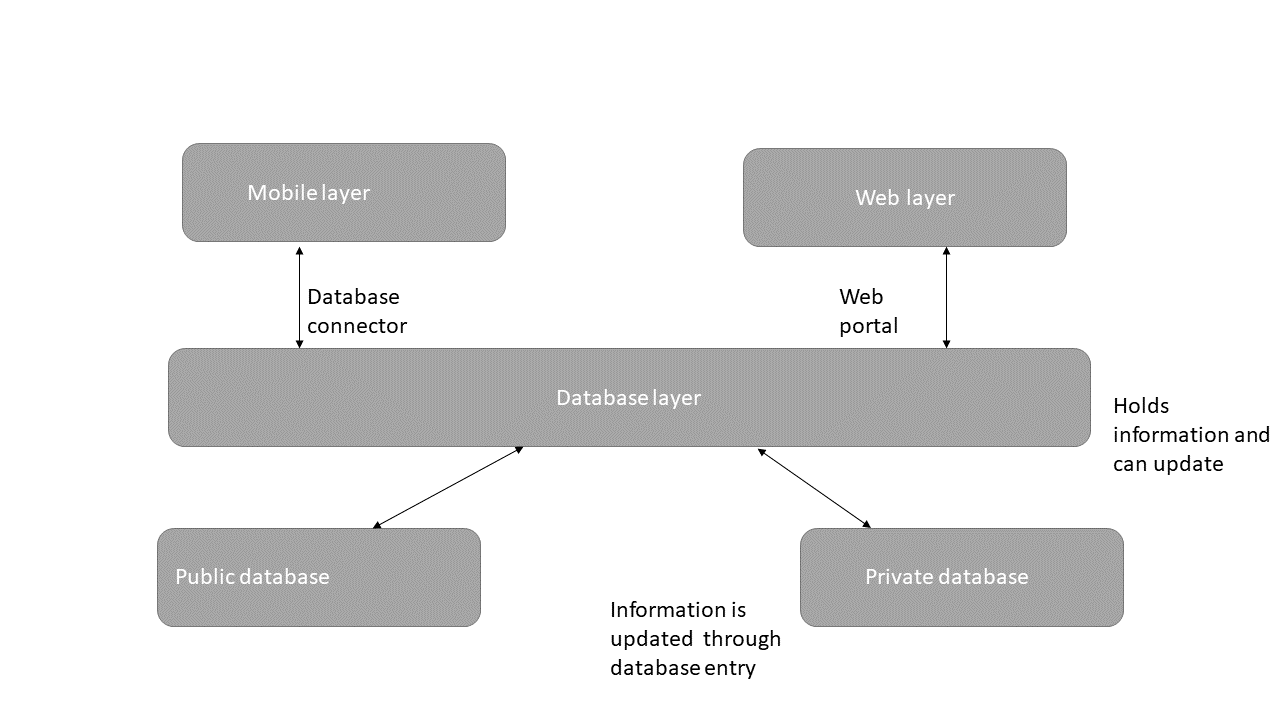
\includegraphics[width=0.60\textwidth]{images/database.pnj}
 \caption{Example subsystem description diagram}
\end{figure}

\subsubsection{Assumptions}
Any assumptions made in the definition of the subsystem should be listed and described. Pay particular attention to assumptions concerning interfaces and interactions with other layers.
When the mobile layer or web layer requests the data or seems to change it from pubic database the database does the required task and displays inthe respected layer or it connects to private database to create or get infromation already created.

\subsubsection{Responsibilities}
Each of the responsibilities/features/functions/services of the subsystem as identified in the architectural summary must be expanded to more detailed responsibilities. These responsibilities form the basis for the identification of the finer-grained responsibilities of the layer's internal subsystems. Clearly describe what each subsystem does.
When the mobile layer or web layer requests the data from public database the database does the required task and displays inthe respected layer
\subsubsection{Subsystem Interfaces}
Each of the inputs and outputs for the subsystem are defined here. Create a table with an entry for each labelled interface that connects to this subsystem. For each entry, describe any incoming and outgoing data elements will pass through this interface.
It will be simitlar to public database used.
\begin {table}[H]
\caption {Subsystem interfaces} 
\begin{center}
    \begin{tabular}{ | p{1cm} | p{6cm} | p{3cm} | p{3cm} |}
    \hline
    ID & Description & Inputs & Outputs \\ \hline
   \#01 & Web portal and databse connector & \pbox{3cm}{local database } & \pbox{3cm}{expanded information \\ on brewery product}  \\ \hline
        \end{tabular}
\end{center}
\end{table}

\subsection{Subsystem 2}
This section should be a general description of a particular subsystem for the given layer. For most subsystems, an extract of the architectural block diagram with data flows is useful. This should consist of the subsystem being described and those subsystems with which it communicates.
This subsytem consist of the private database. So when the web application or mobile layer uses database connectors or the web portal to find the required information if the the inforamtion is not stored in the public database they go to this database which allows to create the required information or the already existinfg one is provided and displayed in the reqiured layer.
\begin{figure}[h!]
	\centering
 	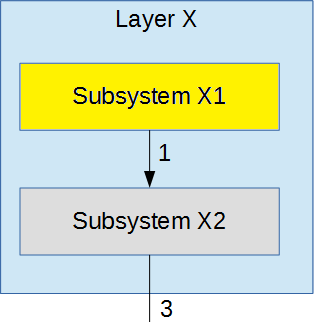
\includegraphics[width=0.60\textwidth]{images/subsystem}
 \caption{Example subsystem description diagram}
\end{figure}

\subsubsection{Assumptions}
Any assumptions made in the definition of the subsystem should be listed and described. Pay particular attention to assumptions concerning interfaces and interactions with other layers.
When the mobile layer or web layer requests the data and is not availbale from pubic database the database does it connects to private database to create or get requested infromation already created in private database.

\subsubsection{Responsibilities}
Each of the responsibilities/features/functions/services of the subsystem as identified in the architectural summary must be expanded to more detailed responsibilities. These responsibilities form the basis for the identification of the finer-grained responsibilities of the layer's internal subsystems. Clearly describe what each subsystem does.
When the mobile layer or web layer requests the data or seems to change it from database layer the database does the required task and displays inthe respected layer
\subsubsection{Subsystem Interfaces}
Each of the inputs and outputs for the subsystem are defined here. Create a table with an entry for each labelled interface that connects to this subsystem. For each entry, describe any incoming and outgoing data elements will pass through this interface.

\subsubsection{Subsystem Interfaces}
Each of the inputs and outputs for the subsystem are defined here. Create a table with an entry for each labelled interface that connects to this subsystem. For each entry, describe any incoming and outgoing data elements will pass through this interface.
It will be simitlar to public database used.
\begin {table}[H]
\caption {Subsystem interfaces} 
\begin{center}
    \begin{tabular}{ | p{1cm} | p{6cm} | p{3cm} | p{3cm} |}
    \hline
    ID & Description & Inputs & Outputs \\ \hline
   \#01 & Web portal and databse connector & \pbox{3cm}{private database } & \pbox{3cm}{expanded information \\ on brewery product}  \\ \hline
        \end{tabular}
\end{center}
\end{table}
